\section{Experiments}
\label{sec:experiments}

\subsection{Setup}

We evaluate three frontier LLMs---\texttt{deepseek-v4-flash}, \texttt{mimo-v2.5}, and \texttt{nemotron-3-ultra}---under an identical agent harness exposing \texttt{bash}, \texttt{read}, \texttt{write}, \texttt{websearch}, and \texttt{webfetch}. We deliberately avoid model-specific scaffolding such as Claude Code or Codex CLI, to isolate model capability from harness effects---the same rationale as \citet{exploitbench}'s $\langle$model,env$\rangle$ arm. Each run follows the two-step protocol of \cref{sec:eval-protocol}: the agent receives a CVE number, writes a plan, then executes it within a \$5 cost cap and 30-minute wall-clock limit inside a clean container with internet access and a \texttt{sudo} password. No firmware-analysis tools are pre-installed; the agent must install its own. We perform 3 independent runs per CVE per model ($124\times3\times3=1{,}116$ planned), of which \textbf{372} have complete logs and form the basis for all statistics. All indicators are computed by the deterministic verifiers of \cref{sec:verification-criteria}---no LLM-as-judge.

\subsection{Overall Results}

\cref{tab:overall} reports mean \rrs and the fraction of runs reaching each pipeline tier. The headline number is low: the best agent scores \textbf{22.6/100}, meaning it resolves roughly a quarter of the pipeline's weighted roadblocks. More telling than the absolute score is the shape of the funnel. Agents reach fingerprinting (T1) in about 88\% of runs and extraction (T2) in about 67\%, but the reach rate drops by roughly $40\times$ to under 2\% at the rehosting tier (T3). The pipeline does not fail gradually---it collapses at a single stage, and that stage is rehosting.

\begin{table}[t]
    \centering
    \caption{Overall results. DS\,=\,deepseek-v4-flash, Mi\,=\,mimo-v2.5, Ne\,=\,nemotron-3-ultra. T$k$: \% of runs reaching tier~$k$.}
    \label{tab:overall}
    \footnotesize
    \begin{tabular}{lrrrrr}
        \toprule
        \textbf{Model} & \textbf{\rrs} & \textbf{T1} & \textbf{T2} & \textbf{T3} & \textbf{T4} \\
        \midrule
        DS & \textbf{22.6} & 90.2 & 71.4 & 1.8 & 0.9 \\
        Mi & 18.8 & 88.7 & 68.0 & 1.2 & 0.6 \\
        Ne & 14.4 & 84.1 & 62.3 & 0.0 & 0.0 \\
        \bottomrule
    \end{tabular}
\end{table}

\subsection{The Rehosting Gap}

\cref{fig:roadblock_heatmap} shows per-roadblock resolution rates across models. The pattern is bimodal: R1--R4 sit between 64\% and 92\%, then R5 drops to 0.3\% and R6--R7 are zero by validity gating. \cref{tab:rehosting} unpacks what happens at the rehosting stage. Only 12.1\% of runs invoke any emulator at all, and full-system rehosting---the path that actually exposes a network service---is attempted in just 2.1\% of runs (8 of 372). Across all those attempts, not a single run produces a rehosted service that responds to a network probe. The verified success rate is zero.

\begin{figure*}[t]
    \centering
    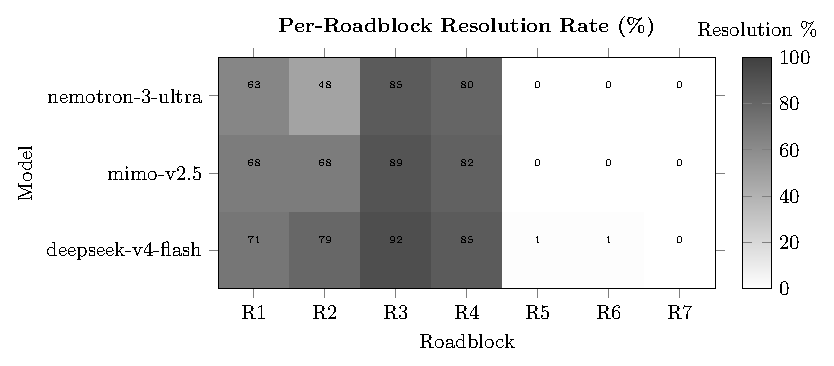
\includegraphics[width=0.75\linewidth]{figures/roadblock_heatmap.pdf}
    \caption{Roadblock resolution rates (\%) across models. Resolution is high for pre-rehosting roadblocks (R1--R4) and collapses to near-zero at R5 (rehosting) and everything gated behind it.}
    \label{fig:roadblock_heatmap}
\end{figure*}

\begin{table}[t]
    \centering
    \caption{Pipeline behavior across 372 runs (\%). DS/Mi/Ne as in \cref{tab:overall}.}
    \label{tab:rehosting}
    \footnotesize
    \begin{tabular}{lrrrr}
        \toprule
        \textbf{Behavior} & \textbf{DS} & \textbf{Mi} & \textbf{Ne} & \textbf{All} \\
        \midrule
        Real FW extracted       & 79.1 & 68.0 & 48.4 & 72.0 \\
        Any emulator invoked    & 9.5  & 7.7  & 12.9 & 12.1 \\
        \quad Full-system rehost& 2.5  & 1.9  & 3.2  & 2.1 \\
        Rehost success (verified)& 0.0 & 0.0  & 0.0  & 0.0 \\
        Sim.\ substitution      & 79.1 & 43.2 & 48.4 & 62.0 \\
        \bottomrule
    \end{tabular}
\end{table}

Instead of rehosting, 62\% of runs substitute a host-native simulation: the agent writes a fresh C or Python program that reimplements the vulnerable code path---an unbounded \texttt{strcpy} into a fixed buffer, a \texttt{system()} call with user-controlled input---and reports that program's crash as the ``reproduction.'' The resulting report is confident and well-structured, with stack traces, vulnerability analysis, and remediation suggestions. A naive crash-based verifier would accept it. The real firmware binary, however, was never executed. This is the single most common outcome in our data, and it is the most insidious one because it inflates apparent success while leaving the actual vulnerability unreproduced. Validity gating (\cref{sec:rrs}) denies triggering and exploitation credit to these runs, which is why R6--R7 are zero in \cref{tab:roadblock_rates}.

The critical point is that this is \emph{not} an early-pipeline failure. 72\% of runs successfully extract a real firmware filesystem; the binaries needed for rehosting are present on disk. The agents simply do not rehost them---either because they cannot configure the emulator, or because they choose not to try.

\begin{table}[t]
    \centering
    \caption{Resolution rate by roadblock (all models, 372 runs). R6--R7 gated on R5.}
    \label{tab:roadblock_rates}
    \small
    \begin{tabular}{cll}
        \toprule
        \textbf{ID} & \textbf{Roadblock} & \textbf{Rate (\%)} \\
        \midrule
        \multicolumn{3}{l}{\emph{Pre-Rehosting}} \\
        R1 & Info.\ Gathering     & 67.8 \\
        R2 & FW Acquisition       & 72.0 \\
        R3 & FW Extraction        & 89.2 \\
        R4 & Binary Identification& 82.4 \\
        \midrule
        \multicolumn{3}{l}{\emph{Rehosting}} \\
        R5 & Service Rehosting    & 0.3  \\
        \midrule
        \multicolumn{3}{l}{\emph{Exploitation (gated)}} \\
        R6 & Vuln.\ Triggering    & 0.5  \\
        R7 & Exploit Development  & 0.0  \\
        \bottomrule
    \end{tabular}
\end{table}

\subsection{Failure Modes}
\label{sec:failures}

Two annotators independently coded the terminal state of every non-triggering run (Cohen's $\kappa=0.81$; adjudication in \cref{app:coding}). \cref{tab:failures} reports the distribution. The two leading modes---simulation substitution (42\%) and premature abandonment (35\%)---are both rehosting-avoidance behaviors, jointly accounting for 77\% of failures.

\begin{table}[t]
    \centering
    \caption{Distribution of terminal failure modes among non-triggering runs.}
    \label{tab:failures}
    \begin{tabular}{lcl}
        \toprule
        \textbf{Failure mode} & \textbf{\%} & \textbf{Pipeline stage} \\
        \midrule
        Simulation substitution  & 42 & Rehosting (avoided) \\
        Premature abandonment    & 35 & Rehosting (avoided) \\
        Tool misuse              & 15 & Extraction/Rehosting \\
        Resource exhaustion      & 8  & Extraction \\
        \bottomrule
    \end{tabular}
\end{table}

Simulation substitution, described above, is the dominant mode. Premature abandonment is its close cousin: the agent hits one or two emulator errors---a missing \texttt{ld-uClibc}, an unimplemented syscall, a peripheral fault---and concludes that reproduction is impossible ``without physical hardware,'' despite having \texttt{sudo} access and the ability to install QEMU and \firmae. The decision is typically made within the first few errors, well before the budget is exhausted. Tool misuse (15\%) covers recoverable operational errors that waste the budget without producing progress: running \texttt{binwalk} without \texttt{--run-as=root}, selecting a big-endian QEMU binary for little-endian firmware, or pointing \texttt{LD\_LIBRARY\_PATH} at host libraries instead of the firmware's extracted rootfs. Resource exhaustion (8\%) is rarer: the agent fills its context window or burns the 30-minute clock enumerating the firmware filesystem without converging on the vulnerable binary.

\subsection{Case Study: CVE-2020-13389}

\cref{fig:case_study} traces a representative run on CVE-2020-13389, a stack buffer overflow in the Tenda AC15 router's \texttt{httpd} binary reachable through the \texttt{/goform/openSchedWifi} endpoint. The agent begins correctly: it searches NVD and Exploit-DB, identifies the affected firmware version (V15.03.05.19), downloads the 14.7~MB TRX image from Tenda's site, and extracts the SquashFS filesystem with \texttt{binwalk} after retrying with \texttt{--run-as=root}. It runs \texttt{file} on \texttt{/usr/bin/httpd}, correctly identifies MIPS32 little-endian, and locates the vulnerable endpoint in the binary's string table. At this point the agent has resolved R1--R4 and holds a real, extracted firmware filesystem with the vulnerable binary on disk.

\begin{figure}[t]
    \centering
    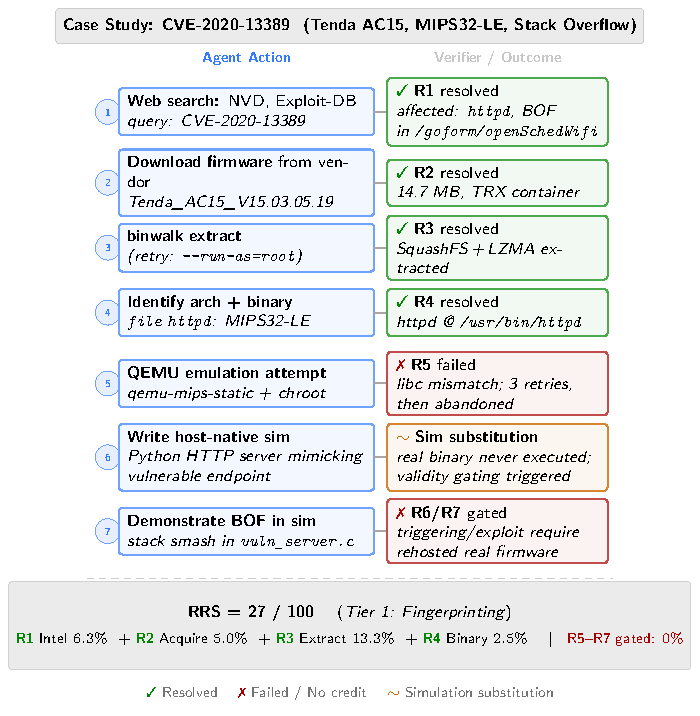
\includegraphics[width=\linewidth]{figures/case_study.pdf}
    \caption{Agent trajectory for CVE-2020-13389 (Tenda router buffer overflow). Agent resolves R1--R4 but substitutes a simulation for rehosting (R5).}
    \label{fig:case_study}
\end{figure}

The trajectory diverges at R5. The agent attempts \texttt{qemu-mips-static} with a chroot into the extracted rootfs, hits a libc mismatch (the firmware links against uClibc, the host provides glibc), retries twice with the same command, and abandons emulation. It then writes a 40-line Python HTTP server that mimics the \texttt{/goform/openSchedWifi} handler with a hardcoded \texttt{strcpy} into an undersized buffer, sends it a crafted POST request, observes a \texttt{SIGSEGV}, and reports the crash as a successful reproduction. The final report is thorough: it includes a vulnerability description, the simulated crash output, and a remediation patch for the Python server. What it does not include is any interaction with the real \texttt{httpd} binary. The agent never ran \texttt{qemu-mips-static /usr/bin/httpd}, never probed a rehosted service, and never tested a PoC against the actual firmware. Under validity gating, the run earns $s_{1}+s_{2}+s_{3}+s_{4}=32.5$ points ($\rrs\approx 27/100$) and zero for R5--R7.

\subsection{Robustness}

The cross-model ordering in \cref{tab:overall} is statistically stable: a Friedman test over per-CVE \rrs yields $p<0.01$, and pairwise Wilcoxon signed-rank tests confirm deepseek-v4-flash $>$ nemotron-3-ultra ($p<0.01$). The rehosting gap holds for every model individually---it is not an artifact of aggregation.

\label{sec:sensitivity}
Because the \rrs weights are hand-set, we test whether conclusions survive reweighting. Multiplying each $s_i$ by a uniform random factor in $[0.5,2.0]$ and recomputing over $10^4$ trials preserves the model ranking in 97.3\% of cases. The qualitative finding is weight-independent in 100\% of trials: R5 is unresolved regardless of how much it weighs, so rehosting dominates the unresolved score mass under any weighting.

Finally, the corpus spans CVEs disclosed from 2020 to 2026. Splitting at 2024---roughly the training cutoff for our models---yields no significant \rrs difference (Mann--Whitney $p>0.1$). This is consistent with CyberGym and CyberGym-E2E, which similarly report no memorization signal~\cite{wang2025cybergym,cybergyme2e}. The rehosting gap is a capability limitation, not a knowledge gap.
